\documentclass{article}
\usepackage{graphicx}
\graphicspath{ {./report_img/} } % graphics path
\usepackage{fancyhdr}
\usepackage{listings}
\setlength{\parindent}{0pt}
\usepackage{float}
\usepackage[letterpaper,margin=1in]{geometry}
\renewcommand{\baselinestretch}{1.2}    % line spacing
\usepackage{amsmath}
\usepackage{amssymb} % for \mathbb -- set of integers
%\usepackage[bf,large]{caption}
\usepackage{caption}
\usepackage{subcaption} % for subfigure environment
\usepackage{steinmetz}  % for \phase
\usepackage{mathrsfs}   % for \mathscr -- Laplace transform operator
\usepackage{mathtools}  % for \floor{}
\usepackage{sectsty}
\usepackage{wrapfig}
\usepackage{lipsum}
\usepackage{hyperref}
\hypersetup{
    colorlinks=true,
    linkcolor=black,
    urlcolor=magenta
}
\usepackage[usenames,dvipsnames]{color}
\definecolor{lightgray}{gray}{0.5}
% This is the color used for MATLAB comments below
\definecolor{MyDarkGreen}{rgb}{0.0,0.4,0.0}
\lstloadlanguages{Matlab, bash}%
\lstset{language=bash,                        % Use MATLAB
        frame=single,                           % Single frame around code
        basicstyle=\small\ttfamily,             % Use small true type font
        %keywordstyle=[1]\color{Blue}\bf,        % MATLAB functions bold and blue
        %keywordstyle=[2]\color{Purple},         % MATLAB function arguments purple
        %keywordstyle=[3]\color{Blue}\underbar,  % User functions underlined and blue
        identifierstyle=,                       % Nothing special about identifiers
                                                % Comments small dark green courier
        commentstyle=\usefont{T1}{pcr}{m}{sl}\color{MyDarkGreen}\small,
        stringstyle=\color{Purple},             % Strings are purple
        showstringspaces=false,                 % Don't put marks in string spaces
        tabsize=2,                              % 5 spaces per tab
        %
        morecomment=[l][\color{Blue}]{...},     % Line continuation (...) like blue comment
        numbers=left,                           % Line numbers on left
        firstnumber=0,                          % Line numbers start with line 1
        numberstyle=\tiny\color{Blue},          % Line numbers are blue
        stepnumber=1,                           % Line numbers go in steps of 5
        breaklines=true
        }
\pagestyle{fancy}
%\thispagestyle{plain}

\def\class{ECE 418}
\def\fp{Final Project Report}

\partfont{\centering}

\lhead{ Sun, Jiang, Shen, \class, \fp}

\begin{document}

\title{\fp}
\date{} % disable date to include in the title
\author{
\begin{tabular}{ccc}
    Alvin Sun & Yuqi Xue & Yan Miao \tabularnewline
    yixiaos3 & yuqixue2 & yanmiao2
\end{tabular}
}
%\maketitle

\begin{titlepage} % Suppresses displaying the page number on the title page and the subsequent page counts as page 1
	\newcommand{\HRule}{\rule{\linewidth}{0.5mm}} % Defines a new command for horizontal lines, change thickness here

	\center % Centre everything on the page

	%------------------------------------------------
	%	Headings
	%------------------------------------------------

	\textsc{\LARGE University of Illinois at Urbana Champaign}\\[1.5cm] % Main heading such as the name of your university/college

	\textsc{\Large ECE 418 Image and Video Signal Processing}\\[0.5cm] % Major heading such as course name

	\textsc{\Large Final Project Report} \\[0.5cm] % Minor heading such as course title

	%------------------------------------------------
	%	Title
	%------------------------------------------------

	\HRule\\[0.6cm]

    {\huge\bfseries Steganography}\\[0.3cm]
    {\huge\bfseries A DCT Approach}\\[0.3cm]
    {\huge\bfseries With Image Hidden Inside Image}\\[0.4cm]

	\HRule\\[1.5cm]

	%------------------------------------------------
	%	Author(s)
	%------------------------------------------------

	\begin{minipage}{0.4\textwidth}
		\begin{flushleft}
			\large
			\textit{Author}\\
			Alvin Sun \\ % Your name
            Bowen Jiang  \\
            Maohao Shen
		\end{flushleft}
	\end{minipage}
	~
	\begin{minipage}{0.4\textwidth}
		\begin{flushright}
			\large
			\textit{Net ID}\\
			yixiaos3 \\ % net id
            bowenj2 \\
            maohaos2
		\end{flushright}
	\end{minipage}

	% If you don't want a supervisor, uncomment the two lines below and comment the code above
	%{\large\textit{Author}}\\
	%John \textsc{Smith} % Your name

	%------------------------------------------------
	%	Date
	%------------------------------------------------

	\vfill\vfill\vfill % Position the date 3/4 down the remaining page

	{\large\today} % Date, change the \today to a set date if you want to be precise

	%------------------------------------------------
	%	Logo
	%------------------------------------------------

	%\vfill\vfill
	%\includegraphics[width=0.2\textwidth]{placeholder.jpg}\\[1cm] % Include a department/university logo - this will require the graphicx package

	%----------------------------------------------------------------------------------------

	\vfill % Push the date up 1/4 of the remaining page

\end{titlepage}

\section{Introduction}

Our project mainly focus on the digital steganography performed on the frequency
domain of colored images, which is also commonly known as the watermarking.
Motivated by the increasing demands of security in massive data transmissions
and digital communications, we designed our project to be able to hide digital
images as the watermark inside larger images as the message to
be transmitted, whose histogram, spatial domain, and frequency domain are all
indistinguishable from the original. To make the following explanation clearer,
we would use the naming convention for the 2 images as below.
\begin{itemize}
    \item \textbf{Carrier Image.} The larger base image that will
        eventually be transmitted or stored to disk.
    \item \textbf{Watermark Image.} The smaller image that is embedded inside
        the Carrier Image. It should not be visible during transmission.
\end{itemize}

\section{Proposed Approach}

Most of the images have their frequency components concentrated in the low
frequency ranges, while details expressed as edges also exist in the very high
freqeuncy range. Therefore, we decided to hide the \textit{watermark image}
into the mid-high frequency regions of the \textit{carrier image}, which has
the least significant impact on the visual effect of the image.

\subsection{General Idea}

\textit{Discrete Cosine Transform} (2D-DCT) is chosen to obtain the frequency domain of the
\textit{carrier image}, other than the Discrete Fourier Transform (2D-DFT),
in order to avoid
the complex number involved in the calculation. Meanwhile, RGB color space is
selected, instead of LAB color space, so that the troublesome nonlinear transformation of
color spaces can be avoided. Any nonlinearity could potentially introduce floating
point truncation errors that could badly hurt the quality of the hidden
\textit{watermark image}.

\subsection{Encoding Stage}

In the encoding stage, the \textit{watermark image} is read directly from an
image file on the disk, which stays with its compressed format (e.g. JPEG, PNG, etc.)
The \textit{carrier image} is also read from the disk, but will be decompressed into raw
RGB pixel format. And then the image will go through normalization such that all pixel
values falls within $[0,1]$. Then, we iterate through a predetermined rectangle
range in the mid-high frequency region of the frequency domain of the
\textit{carrier image}. The iteration also scans through the 3 RGB channels as it
progresses. Every iteration, when the magnitude of a frequency component is less
than a pre-determined threshold, we encode one data byte from the
\textit{watermark image} into the magnitude of that freqeuncy value, which means
its sign is preserved. The encoding is not a direct assignment as the normalization
cause the average magnitude of the freqeuncy component to be quite small. Instead,
we multiple the byte value with a pre-defined scale and then assign this scaled value
to the magnitude of the frequency component. The smaller the scale it is, the smaller
the visual impact this freqeuncy domain operation could cause, but also the less
significant it has on the spatial domain pixel values. As a result, we need a
16-bit quantization instead of 8-bit to preserve the fine details we modified inside
the freqeuncy domain. In addtion to encoding the image data
itself, we also needs to know the total length of the \textit{watermark image} byte
stream for the decoding stage, so we encode this length information as a 4-byte unsigned
integer using the same scheme as encoding the data, but at a pre-determined location
within the DCT image. Figure \ref{fig:encoder} shows a general work flow of the
encoding stage.

\begin{figure}[h]
    \centering
    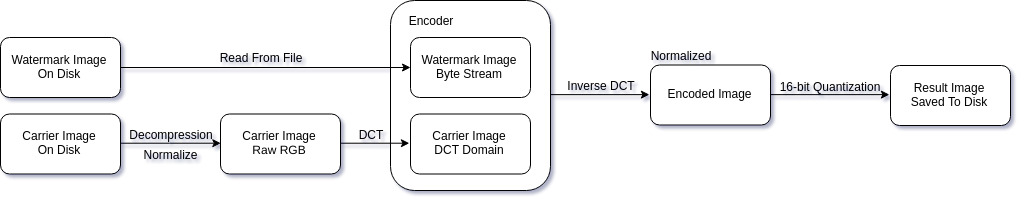
\includegraphics[width=\textwidth]{encoder}
    \caption{Encoder Diagram}
    \label{fig:encoder}
\end{figure}

\subsection{Decoding Stage}

In the decoding stage, the whole process is not very different but just the
reverse of the encoding stage. As we iterate through the rectangle region and
three color channels, if the current frequency magnitude is lower than the
predetermined threshold, we can divide the magnitude by the predetermined scale
and then round it to the neareast integer value to extract the original
\textit{watermark image} bytes, until the number of bytes retrieved matches the
length we extract at the very beginning from a pre-determined location. After
the complete byte array is obtained, the data will be transformed back to the
colored image through image decompression based on its original format. Figure
\ref{fig:decoder} shows a general work flow of the decoding stage.

\begin{figure}[h]
    \centering
    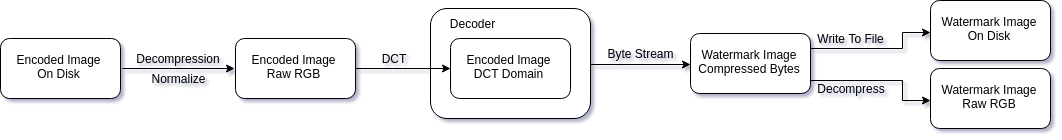
\includegraphics[width=\textwidth]{decoder}
    \caption{Decoder Diagram}
    \label{fig:decoder}
\end{figure}

\section{Experimental Design And Results}

\subsection{Carrier Image Choice}

\begin{wrapfigure}{r}{0.61\textwidth}
    \centering
    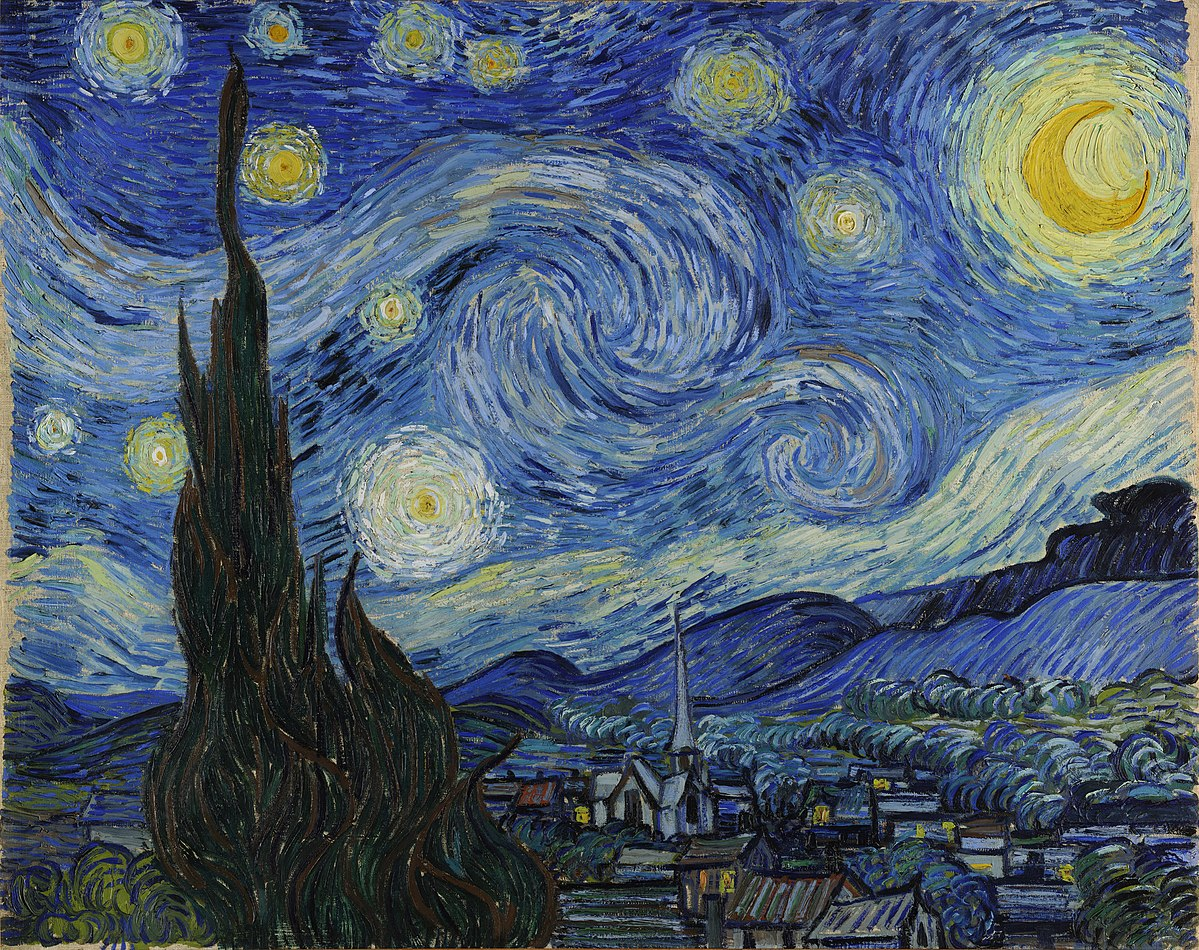
\includegraphics[width=0.40\textwidth]{starry_night}
    \caption{Carrier Image}
    \label{fig:starry}
\end{wrapfigure}

We implemented and experimented with a carrier image shown in Figure
\ref{fig:starry}, which has many high frequency components. This will be
especially challenging for us to test the robustneses of our steganography
algorithm as we are potentially modifying quite an amount of mid-high freqeuncy
component of the original \textit{carrier image}. This also helps us visualize
the actual impact on the visual impression of the \textit{carrier image} when
embedding the \textit{watermark image} inside.

\subsection{DCT of Carrier Image}

Shown in Figure \ref{fig:dct_original} is the DCT domain of the 3 RGB channels of
the original \textit{carrier image}. The values are truncated to enhance the contrast
for the purpose of visulization. As we can see from the images, most information
is concentrated in the low frequency region, while high freqeuncy components also
occupy a decent portion of the total energy.

\begin{figure}[h]
    \centering
    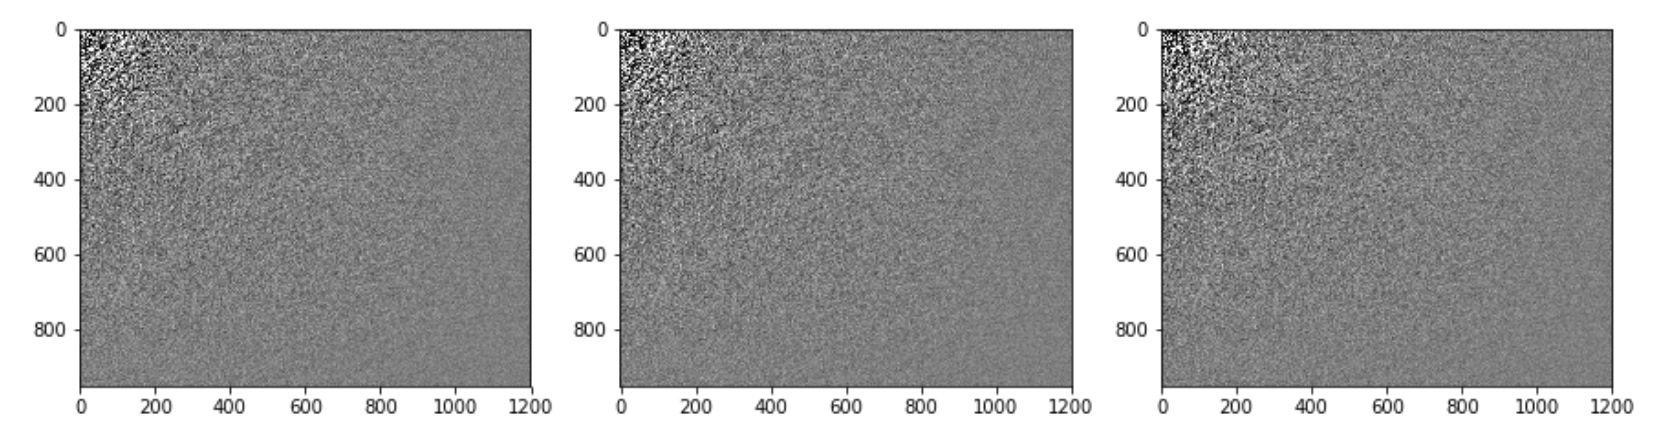
\includegraphics[width=\textwidth]{dct_original}
    \caption{DCT of The Original Carrier Image}
    \label{fig:dct_original}
\end{figure}

\subsection{Watermark Image Choice}

Because the maximum length of data bytes that can be encoded is bounded by
the size of the rectangle region we pick in the frequency domain, we cannot
hide very large sized image within the \textit{carrier image}. Therefore, we
picked the resized picture shown in Figure \ref{fig:small} as our \textit{watermark
image} to experiment with.

\begin{figure}[h]
    \centering
    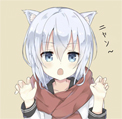
\includegraphics[width=0.25\textwidth]{small}
    \caption{Watermark Image}
    \label{fig:small}
\end{figure}

\subsection{Encoding / Decoding Results}

After the encoding stage, the inverse DCT gives us the following result as shown
in Figure \ref{fig:starry_encoded}, which looks indistinguishable from the
original image before the encryption. Then we put this encoded image to our decoder,
and we extracted back the \textit{watermark image} with absolutely no attenuation.
In other words, the recoverage of hidden information is perfect. Figure
\ref{fig:decoded_small} is the extracted hidden \textit{watermark image} from the encoded
\textit{carrier image}. Again, we can see that it is pixel-wise identical to the
original \textit{watermark image}.

\begin{figure}[h]
    \centering
    \begin{subfigure}[t]{0.6\textwidth}
        \includegraphics[width=\textwidth]{encoded}
        \caption{Encoded Carrier Image}
        \label{fig:starry_encoded}
    \end{subfigure}
    ~
    \begin{subfigure}[t]{0.35\textwidth}
        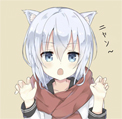
\includegraphics[width=\textwidth]{decoded}
        \caption{Decoded Watermark Image}
        \label{fig:decoded_small}
    \end{subfigure}
    \caption{Encoder / Decoder Results}
\end{figure}

\subsection{Histogram Analysis}
We have also compare the histogram of the image before and after watermarking,
and the result shows that it is unobvious to discover that the \textit{carrier image}
has been watermarked. Figure \ref{fig:histogram} shows the the 2 histograms.

\begin{figure}[h]
    \centering
    \begin{subfigure}[t]{0.48\textwidth}
        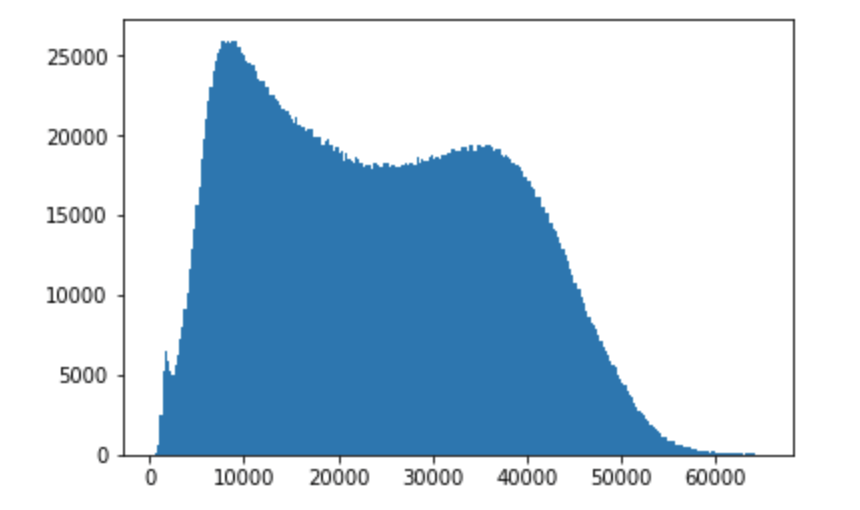
\includegraphics[width=\textwidth]{hist_original}
        \caption{Histogram of Original Image}
    \end{subfigure}
    \begin{subfigure}[t]{0.48\textwidth}
        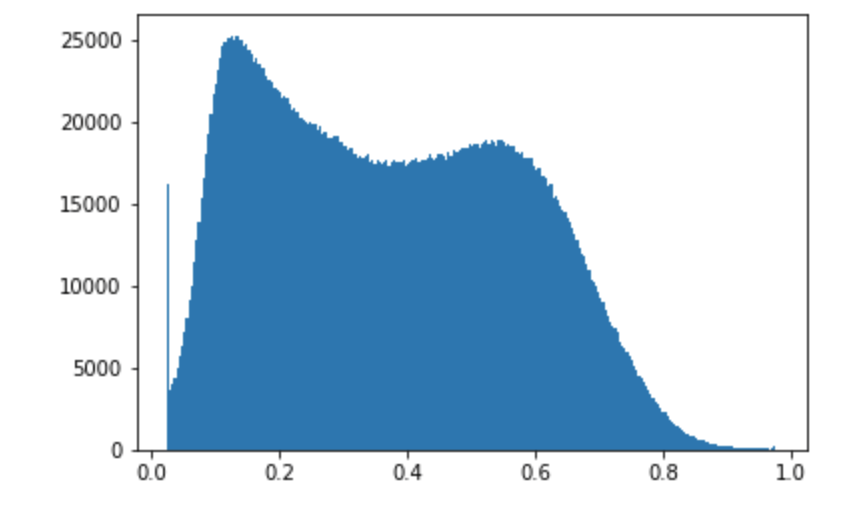
\includegraphics[width=\textwidth]{hist_water}
        \caption{Histogram of Watermarked Image}
    \end{subfigure}
    \caption{Encoder / Decoder Results}
    \label{fig:histogram}
\end{figure}

\section{Discussion And Future Work}

In summary, the result of this project reached our expectation. At the beginning,
we decided to implement steganography for text message, but we soon tried to
improve it to hide small image into large image, which is more robust and
add an additional level of indirection to the message we would like to hide. \\

Our steganography can hide any type of digital information inside large colored images
in the form of high frequency components within DCT domain. Meanwhile, the whole
encryption process can not be discovered from the spatial domain image,
frequency domain image, or the pixel statistics such as histograming. This
ensures the security of the hidden message or image. \\

That being said, there still exist some shortcomings as well. For example, the
watermark image is of limited size and definition. Also, the encoder and decoder
needs to agree on quite a large number of pre-determined constants to have a perfect
reconstruction of the hiddle information. We still have some ideas to improve
this project. Considering the security level, we can encode the message into
random locations of large image, instead of in a fixed rectangle region. To
implement this, we need a pseudo-random function with a seed, which generates
pseudo-random locations for message encoding, while using the same seed in
decoding process. This improvement will be able to make this project more secure
and reliable, since no one could find the difference in frequency domain even
though someone else may try to find regularity based on large amounts of encoded
images. Another relatively tricky improvement is real time steganography. we may
try to encode message or small images in video such as video chat. This process
may require processing a lot of data and we also need consider the temporal
domain effect.

\section*{Appendix}

Our code is open source and is developed in Python 3.6, which is available
\href{https://github.com/alvinsunyixiao/ece418-stenography}{HERE}. To use
the encoder / decoder program, simply run
\begin{lstlisting}[language=bash]
    python3 encode.py <carrier_img> <watermark_img> # for encoding
    python3 decode.py <encoded_img> # for decoding
\end{lstlisting}
\textbf{Note.} To run the program, you may need to look into the source code
and get the prerequisite package installed beforehand.




\end{document}
